\documentclass[11pt,reqno]{amsart}

\usepackage{amsmath,amsthm,amssymb}
\usepackage{mathtools}
\usepackage{hyperref}
\hypersetup{
  colorlinks=true,
  linkcolor=blue!50!black,
  citecolor=blue!50!black,
  urlcolor=blue!60!black
}
\usepackage{listings}
\usepackage{xcolor}
\usepackage{array}
\usepackage{booktabs}
\usepackage{geometry}
\usepackage{tikz}
\usetikzlibrary{arrows.meta,positioning,fit,calc}
\geometry{margin=1in}
\setlength{\emergencystretch}{3em}

\lstset{
  basicstyle=\small\ttfamily,
  breaklines=true,
  columns=fullflexible,
  keepspaces=true,
  frame=single,
  framesep=4pt,
  rulecolor=\color{black!30},
  showstringspaces=false,
  aboveskip=6pt,
  belowskip=6pt
}

\newtheorem{theorem}{Theorem}[section]
\newtheorem{proposition}[theorem]{Proposition}
\newtheorem{lemma}[theorem]{Lemma}
\newtheorem{corollary}[theorem]{Corollary}
\theoremstyle{definition}
\newtheorem{definition}[theorem]{Definition}
\newtheorem{remark}[theorem]{Remark}

\newcommand{\CombArg}{\texttt{CombArg}}
\newcommand{\Mathlib}{\texttt{Mathlib}}
\newcommand{\unit}{\mathbf{I}}
\newcommand{\NC}{\mathrm{NC}}
\newcommand{\leanrepo}{https://github.com/MathNetwork/comb_arg/blob/v0.1.0/CombArg}
% Clickable Lean declaration tags — verified-green with checkmark.
% \normalfont inside each tag forces upright texttt even when the
% enclosing theorem body is italic (amsthm default).
\definecolor{leangreen}{HTML}{2E7D32}
% Inline clickable tag.
%   \lean{short_name}{File/Path.lean}
\newcommand{\lean}[2]{{\normalfont\color{leangreen}%
  \ensuremath{\checkmark}\,\href{\leanrepo/#2}{\texttt{#1}}}}
% Header tag: small right-flushed bracketed name with checkmark,
% rendered right after the theorem/def/prop label.
%   \leanmargin{short_name}{File/Path.lean}
\newcommand{\leanmargin}[2]{%
  \nopagebreak\hfill{\normalfont\small\color{leangreen}%
    [\ensuremath{\checkmark}\,\href{\leanrepo/#2}{\texttt{#1}}]}\par\nopagebreak
}
% Two-decl header tag, comma-separated on one line.
\newcommand{\leanmargintwo}[4]{%
  \nopagebreak\hfill{\normalfont\small\color{leangreen}%
    [\ensuremath{\checkmark}\,\href{\leanrepo/#2}{\texttt{#1}},
     \ensuremath{\checkmark}\,\href{\leanrepo/#4}{\texttt{#3}}]}\par\nopagebreak
}

\title{Compiling the Almgren--Pitts Combinatorial Argument}

\author{Xinze Li}
\thanks{\textit{Correspondence:} \texttt{lixinze@math.utoronto.ca}}
\date{\today}

\begin{document}

\begin{abstract}
The Almgren--Pitts combinatorial argument is a recurring
technical step in min-max constructions of embedded minimal
hypersurfaces: a cover-refinement on the parameter interval,
followed by a bookkeeping argument that turns local near-critical
savings into a global supremum improvement. Each author
re-derives it in local notation. We extract it from the
literature as a standalone metric-combinatorial algorithm and
formalize it in Lean~4 as the importable library \CombArg.
\end{abstract}

\maketitle

\section{Introduction}
\label{sec:intro}

A minimal hypersurface is a critical point of the area functional
in codimension one. On a closed Riemannian manifold
$(M^{n+1}, g)$, direct minimization over a fixed homology class
may produce only degenerate configurations, and the relevant
critical points are typically of saddle type. The resolution,
following Birkhoff (1917) for closed geodesics and Almgren--Pitts
for higher-dimensional varifolds, is a \emph{min-max}
construction; regularity of the output is Schoen--Simon~\cite{SS81}.

\begin{theorem}[Almgren--Pitts min-max theorem~\cite{Pit81,SS81}]
\label{thm:minmax}
Every closed Riemannian manifold $(M^{n+1}, g)$ admits a
nontrivial embedded minimal hypersurface $\Sigma \subset M$ whose
singular set $\mathrm{Sing}\,\Sigma$ has Hausdorff dimension at
most $n - 7$.
\end{theorem}

The core technical result of Pitts's proof, used in every
subsequent treatment~\cite{CDL03,DLT13,DLR17,DL12,MN14}, is the
Almgren--Pitts combinatorial argument, stated in the
Colding--De~Lellis formulation as follows.

\begin{theorem}[Almgren--Pitts combinatorial Argument,
{\cite[Prop.~3.4]{CDL03}}]
\label{thm:AP-combinatorial}
Let $\Lambda$ be a homotopically closed family of sweepouts of
$M^{n+1}$, and $m_0 = \inf_\Lambda \mathcal{F}$. There exists a
min-max sequence $\{\Gamma^N\}$ converging as varifolds to a
stationary integral varifold of mass $m_0$, with $\Gamma^N$
$1/N$-almost-minimizing in every pair
$(U^1, U^2) \in \mathcal{CO}$ of $\mathcal{H}^n$-disjoint open
sets, for all $N$ sufficiently large.
\end{theorem}

The proof of Theorem~\ref{thm:AP-combinatorial} reduces to
a one-parameter claim on the sweepout~\cite[\S3.2]{DLT13}:

\begin{quote}
\textbf{Claim.} For each $N$ sufficiently large, there exists
$t_N \in [0,1]$ such that $\Gamma^N := \Gamma^N_{t_N}$ is
$1/N$-almost-minimizing in every $(U^1, U^2) \in \mathcal{CO}$
and $\mathcal{H}^n(\Gamma^N) \ge m_0 - 1/N$.
\end{quote}

The Claim is proved by contradiction: from its negation, every
$t$ with $\mathcal{H}^n(\partial \Omega^N_t) \ge m_0 - 1/N$
admits a \emph{local replacement} with saving $1/(4N)$
\cite[Lemma~3.1]{DLT13}; a combinatorial cover-refinement and
bookkeeping argument on $[0,1]$ then assembles from these local
replacements a modified sweepout with supremum strictly below
$m_0$,
contradicting $m_0 = \inf_\Lambda \mathcal{F}$. The combinatorial
argument depends on no geometric measure theory, no admissible
class, and no ambient regularity; it is a bookkeeping
construction on continuous real-valued functions, yet has no
canonical reference.

The scalar formulation of the proof of the Claim, which is the
precise theorem we formalize, reads as follows.

\begin{theorem}[Extracted scalar version]
\label{thm:intro-scalar}
Let $X$ be a pseudo-metric space with an abstract paired-cover
structure. Let $f : [0,1] \to \mathbb{R}$ be continuous with
$m_0 = \sup f$ and $m_0 > 0$, and let $N \in \mathbb{N}$ with
$N > 0$. Suppose that at every $t \in [0,1]$ with
$f(t) \ge m_0 - 1/N$ there is a \emph{local witness}: an open
neighborhood $U_t \ni t$, a paired cover $c_t$ in $X$, and a
continuous replacement energy $E_t : [0,1] \to \mathbb{R}$
satisfying $f(s) - E_t(s) \ge 1/(4N)$ for every $s \in U_t$.
Then there exists $f' : [0,1] \to \mathbb{R}$ with
\[
\sup f' \;\le\; m_0 - \frac{1}{4N}.
\]
\end{theorem}

Translation from the De~Lellis--Tasnady setting to Theorem~\ref{thm:intro-scalar}:
the boundary $\partial \Omega_t$ becomes a continuous
$f : [0,1] \to \mathbb{R}$; the Hausdorff-measure hypothesis
becomes $m_0 = \sup f$; the nested pair $(A_t, B_t, U_t')$
collapses to a single neighborhood $U_t$; the replacement family
$\{\partial \Omega_{t,\tau}\}$ collapses to a single continuous
$E_t$; and the almost-minimizing hypothesis is no longer needed.

The Lean library actually proves a more general statement, of
which Theorem~\ref{thm:intro-scalar} is a direct specialization:
the parameter interval $[0,1]$ may be replaced by any compact,
nonempty topological space $K$, and the specific pair
$(1/N, 1/(4N))$ by arbitrary scalars $(\delta, \varepsilon)$ with
$0 < \varepsilon \le \delta$. The input is then a finite covering
of the $\delta$-super-level set of $f$ carrying per-piece
replacements with uniform saving $\varepsilon$.

\begin{theorem}[Abstract core]
\label{thm:intro-core}
Let $K$ be a compact, nonempty topological space, $f : K \to
\mathbb{R}$ a continuous energy with $m_0 = \sup f$, and let
$0 < \varepsilon \le \delta$. Suppose there is a finite family of
pieces $\{p_l \subseteq K\}_{l \in \iota}$, replacement energies
$\{E_l : K \to \mathbb{R}\}$, and savings
$\{s_l \ge \varepsilon\}$ with: (I) $f - E_l \ge s_l$ on $p_l$;
(II) every $t \in K$ lies in at most two pieces; (III)
$\{t \in K : f(t) \ge m_0 - \delta\} \subseteq \bigcup_l p_l$.
Then there exists $f' : K \to \mathbb{R}$ with
\[
\sup f' \;\le\; m_0 - \varepsilon.
\]
\end{theorem}

Theorem~\ref{thm:intro-scalar} follows by taking $K = [0,1]$,
$\delta = 1/N$, $\varepsilon = 1/(4N)$, and running a 1D
cover-refinement construction on the local witnesses to produce
the family $\{p_l\}$ with two-fold overlap. Both theorems reappear
in §\ref{sec:spec}: Theorem~\ref{thm:intro-core} as the library's
abstract API (Theorem~\ref{thm:core},
\S\ref{sec:core-spec}), and Theorem~\ref{thm:intro-scalar} as the
one-parameter application (Theorem~\ref{thm:main},
\S\ref{sec:app-spec}).

\textbf{Scope.} This note formalizes the proof of the Claim
(the combinatorial argument on $[0,1]$) as a Lean 4 library,
\CombArg. We do \emph{not}
formalize \cite[Lemma~3.1]{DLT13} (the replacement family), the
$(U^1, U^2) \in \mathcal{CO}$ disjoint-pair structure, or the
final contradiction against $m_0 = \inf_\Lambda \mathcal{F}$;
these depend on the GMT and admissible-class framework of the
ambient construction and remain the consumer's responsibility.
The library ships a single abstract theorem
(§\ref{sec:core-spec}) parametric in the sweepout space together
with a one-parameter specialization to $[0,1]$
(§\ref{sec:app-spec}); the formalization is machine-verified
against \Mathlib, declares no custom axioms, and contains no
\texttt{sorry}. Source:
\url{https://github.com/MathNetwork/comb_arg}.

\section{Specification}
\label{sec:spec}

We present the library specification following standard software
documentation conventions: interface first
(\S\ref{sec:interface}), public API
(\S\ref{sec:core-spec}--\S\ref{sec:app-spec}), internal lemmas
(\S\ref{sec:internal}).

\subsection{Interface: types and structures}
\label{sec:interface}

Throughout, \texttt{K} denotes a topological space (the parameter
space), \texttt{X} a pseudo-metric space (the ambient space whose
covers witness replacements), and \texttt{f : K $\to$ $\mathbb{R}$}
a continuous scalar energy.

In the proof of Theorem~\ref{thm:AP-combinatorial}, the
Lemma~3.1 of~\cite{DLT13} supplies, for each near-critical
parameter $t$, an $\mathcal{H}^n$-disjoint pair of open sets
$(U_{1,t}', U_{2,t}')$ in $M^{n+1}$ inside which a local
replacement is performed. We abstract this pair as an instance of
a class, stripped of its GMT content.

\begin{definition}[\texttt{PairableCover} class]
\label{def:pcover}
\leanmargin{PairableCover}{Witness.lean}
A \texttt{PairableCover X} instance declares, for each abstract
\texttt{c : Cover}, a left region and a right region in $X$ and a
scalar diameter, subject to two axioms: the two regions are
disjoint, and overlapping combined regions of diameter-comparable
covers are ordered by inclusion.
\end{definition}

The replacement family
$\{\partial \Omega_{t,\tau}\}_{\tau \in [0,1]}$ at a near-critical
$t$ has its Hausdorff measure decreased by at least $1/(4N)$
inside $U_t'$. We keep only the scalar \emph{replacement energy}
$E : K \to \mathbb{R}$ and the uniform saving inequality; the
geometric family is discarded.

\begin{definition}[\texttt{LocalWitness} structure]
\label{def:witness}
\leanmargin{LocalWitness}{Witness.lean}
A \texttt{LocalWitness K X f t $\varepsilon$} carries an open
neighborhood $U \ni t$ in $K$, a cover \texttt{c : Cover}, a
continuous replacement energy $E : K \to \mathbb{R}$, and the
inequality $\forall s \in U,\; f(s) - E(s) \ge \varepsilon$.
\end{definition}

The proof of the Claim works on the set $K \subset [0,1]$ of
parameters at which the sweepout is within $1/N$ of the min-max
value. We use the same convention.

\begin{definition}[Near-critical set]
\label{def:NC}
\leanmargin{nearCritical}{Refinement/InitialCover.lean}
For continuous $f : K \to \mathbb{R}$, scalar $m_0$, and
$\delta \ge 0$, the $\delta$-near-critical set is
$\{t \in K : f(t) \ge m_0 - \delta\}$. When $\delta = 1/N$ we
write $\NC$.
\end{definition}

At the end of the refinement the data is a family
$\{\overline{J_l}\}$ covering $K$, with each $J_l$ carrying a
replacement whose energy saving is at least $1/(4N)$ and with
two-fold overlap. We abstract this output: the near-critical
threshold $1/N$ becomes a parameter $\delta$ and the saving floor
$1/(4N)$ a parameter $\varepsilon \le \delta$.

\begin{definition}[\texttt{FiniteCoverWithWitnesses} structure]
\label{def:ref}
\leanmargin{FiniteCoverWithWitnesses}{Core.lean}
A \texttt{FiniteCoverWithWitnesses K f m\textsubscript{0} $\delta$ $\varepsilon$}
carries a finite nonempty index type $\iota$, pieces
$\{p_l \subseteq K\}_{l \in \iota}$, replacement energies
$\{E_l : K \to \mathbb{R}\}$, and savings
$\{s_l \in \mathbb{R}_{>0}\}$, subject to four conditions:
(I) $f - E_l \ge s_l$ on $p_l$;
(II) each $t \in K$ lies in at most two pieces;
(III) $s_l \ge \varepsilon$ for all $l$;
(IV) $\{t \in K : f(t) \ge m_0 - \delta\} \subseteq \bigcup_l p_l$.
\end{definition}

Before the refinement, a Lebesgue-number argument on the
compact set $K$ produces a finite covering $\{I_i\}$ of open
intervals, each centered at a $t_i \in K$. In our formalization
the interval center $c_i$ and the witness center $w_i$ are
recorded separately: grid points need not themselves lie in $K$.

\begin{definition}[\texttt{InitialCover} structure]
\label{def:ic}
\leanmargin{InitialCover}{Refinement/InitialCover.lean}
Specialized to $K = \unit$. An
\texttt{InitialCover X f m\textsubscript{0} N} carries a finite
family of open intervals $I_i = (c_i - r_i, c_i + r_i) \cap \unit$
for $i = 1, \ldots, n$, each paired with a witness center
$w_i \in \NC$ and a local witness at $w_i$ with saving $1/(4N)$,
subject to
(a) spacing: $c_i + r_i < c_{i+2} - r_{i+2}$ for all valid $i$;
(b) containment: $I_i \subseteq U_{w_i}$;
(c) coverage: $\NC \subseteq \bigcup_i I_i$.\footnote{Conditions
(a) and (b) transcribe the spacing and subset conditions of the
original proof.}
\end{definition}

The refinement is described as an iteration: each $I_j$ with
$j \ge 2$ is either kept whole or split into two halves. The
state of this iteration after $\ell$ moves is the following.

\begin{definition}[\texttt{PartialRefinement} structure]
\label{def:pr}
\leanmargin{PartialRefinement}{Refinement/PartialRefinement.lean}
Given \texttt{ic : InitialCover} and $\ell \in \mathbb{N}$, a
\texttt{PartialRefinement ic $\ell$} carries pieces
$J_1, \ldots, J_\ell \subseteq \unit$ and an index assignment
$\sigma : \{1, \ldots, \ell\} \to \{1, \ldots, n\}$ with
(i) $J_k \subseteq I_{\sigma(k)}$ for each $k$;
(ii) $I_{\sigma(k)} \subseteq \bigcup_{k'} J_{k'}$ for each $k$.
\end{definition}

\subsection{Public API: abstract core}
\label{sec:core-spec}

\begin{theorem}[Abstract core]
\label{thm:core}
\leanmargin{exists\_sup\_reduction\_of\_cover}{Core.lean}
\noindent
\textbf{Input.} A compact, nonempty topological space $K$; a
continuous $f : K \to \mathbb{R}$; $m_0 = \sup f$; scalars
$0 < \varepsilon \le \delta$; a
\texttt{FiniteCoverWithWitnesses}$(K, f, m_0, \delta, \varepsilon)$
(Definition~\ref{def:ref}).

\par\noindent
\textbf{Output.} There exists $f' : K \to \mathbb{R}$ with
$\sup f' \le m_0 - \varepsilon$.
\end{theorem}

\subsection{Public API: one-parameter application}
\label{sec:app-spec}

\begin{theorem}[One-parameter application]
\label{thm:main}
\leanmargin{exists\_sup\_reduction}{SupReduction.lean}
\noindent
\textbf{Input.} A pseudo-metric space $X$ with a
\texttt{PairableCover X} instance (Definition~\ref{def:pcover});
a continuous $f : \unit \to \mathbb{R}$; $m_0 \in \mathbb{R}$
with $m_0 > 0$ and $m_0 = \sup f$; $N \in \mathbb{N}$ with
$N > 0$; for every $t \in \NC$ a \texttt{LocalWitness} at $t$
with saving $1/(4N)$ (Definition~\ref{def:witness}).

\par\noindent
\textbf{Output.} There exists $f' : \unit \to \mathbb{R}$ with
$\sup f' \le m_0 - 1/(4N)$.

\par\noindent
Specializes Theorem~\ref{thm:core} to $K = \unit$,
$\delta = 1/N$, $\varepsilon = 1/(4N)$.
\end{theorem}

\subsection{Internal lemmas}
\label{sec:internal}

The declarations below are consumed by Theorem~\ref{thm:main};
proofs are sketched in \S\ref{sec:proof}.

\begin{proposition}[Compactness of $\NC$]
\label{prop:NC-compact}
\leanmargintwo{isCompact\_nearCritical}{Refinement/InitialCover.lean}%
              {nearCritical\_nonempty}{Refinement/InitialCover.lean}
If $K$ is compact and $f$ continuous, $\NC$ is compact. If
additionally $m_0 = \sup f$ and $N > 0$, $\NC$ is nonempty.
\end{proposition}

\begin{itemize}
\item \lean{exists\_initialCover}{Refinement/CoverConstruction.lean}
: existence of an \texttt{InitialCover} via a grid plus
Lebesgue-number construction on the compact sublevel set $\NC$.
\item \lean{exists\_terminal\_refinement}{Refinement/Induction.lean}
: existence of a terminal \texttt{PartialRefinement} with
injective $\sigma$ via bounded smallest-index induction with
two-case dispatch.
\item \lean{not\_three\_overlap}{Refinement/Disjointness.lean}
: at most two among any three distinct \texttt{InitialCover}
intervals overlap at a common point (parity rescue).
\item \lean{saving\_bound\_closure}{Refinement/Assembly.lean}
: the open-neighborhood saving bound in \texttt{LocalWitness}
extends to the closure via continuity of $E$.
\item \lean{exists\_refinement}{Refinement/Assembly.lean}
: packages the 1D construction output as a
\texttt{Finite\discretionary{-}{}{}Cover\discretionary{-}{}{}With\discretionary{-}{}{}Witnesses}
with $(\delta, \varepsilon) = (1/N, 1/(4N))$ on $\unit$; the input
to Theorem~\ref{thm:core}.
\end{itemize}

Figure~\ref{fig:arch} shows the layered architecture.

\begin{figure}[tb]
\centering
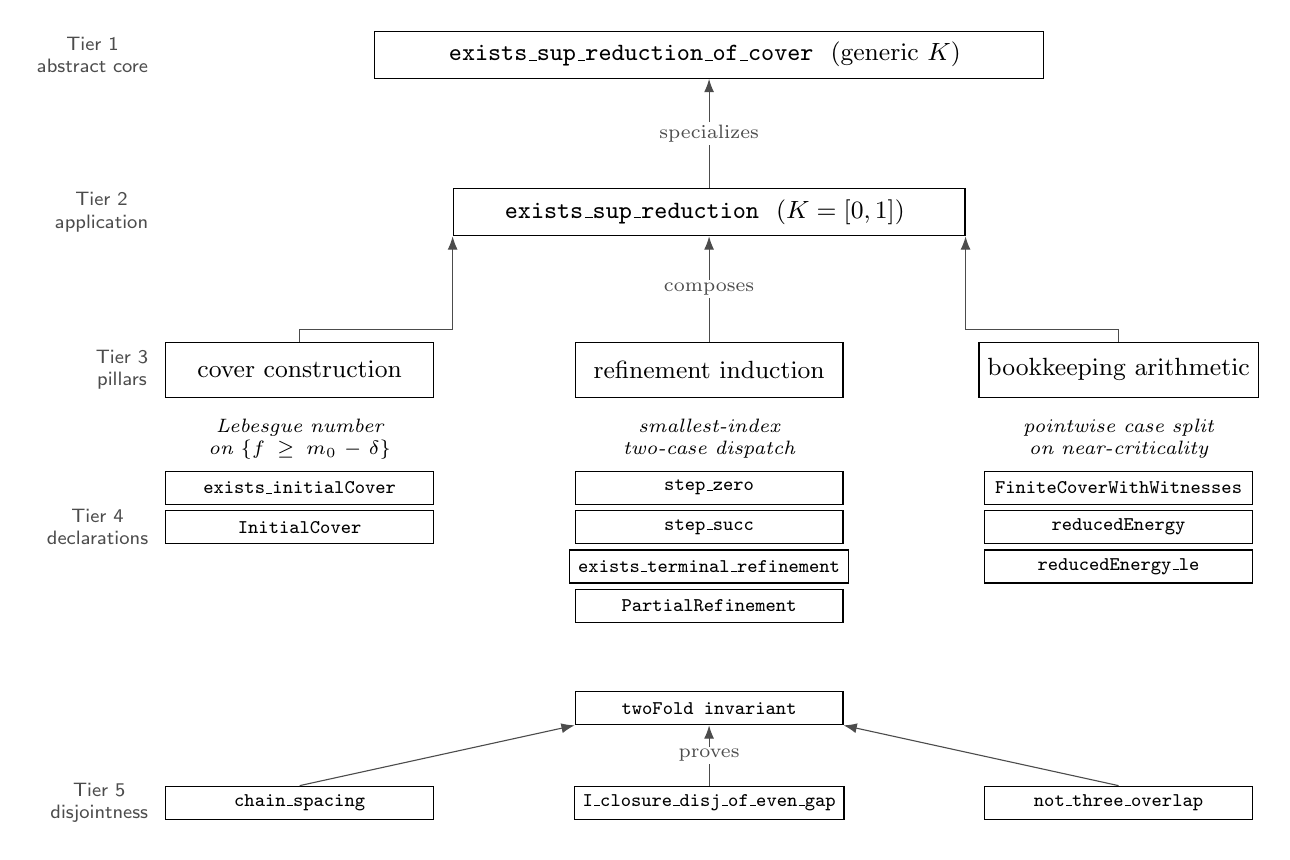
\begin{tikzpicture}[
  font=\small,
  every node/.style={align=center},
  box/.style={draw=black, thin, rectangle, inner sep=3pt, minimum height=6mm},
  pillar/.style={box, minimum width=34mm, minimum height=7mm},
  decl/.style={box, font=\scriptsize\ttfamily, minimum width=34mm, minimum height=4.2mm, inner ysep=1.5pt},
  note/.style={font=\scriptsize\itshape, text width=34mm, align=center, anchor=north},
  tierlbl/.style={font=\sffamily\scriptsize, anchor=east, text=black!70},
  arr/.style={-Latex, thin, black!70},
  arrlab/.style={font=\scriptsize, midway, fill=white, inner sep=1pt, text=black!70}
]

% Tier 1: abstract core
\node[box, minimum width=85mm] (core) at (0, 8) {%
  \texttt{exists\_sup\_reduction\_of\_cover} \ (generic $K$)
};
\node[tierlbl] at (-7, 8) {Tier 1\\abstract core};

% Tier 2: one-parameter application
\node[box, minimum width=65mm] (app) at (0, 6) {%
  \texttt{exists\_sup\_reduction} \ ($K = [0,1]$)
};
\node[tierlbl] at (-7, 6) {Tier 2\\application};
\draw[arr] (app) -- node[arrlab] {specializes} (core);

% Tier 3: three pillars
\node[pillar] (P1) at (-5.2, 4) {cover construction};
\node[pillar] (P2) at ( 0,   4) {refinement induction};
\node[pillar] (P3) at ( 5.2, 4) {bookkeeping arithmetic};
\node[tierlbl] at (-7, 4) {Tier 3\\pillars};
\draw[arr] (P1.north) -- ++(0,0.15) -| (app.south west) ;
\draw[arr] (P2.north) -- node[arrlab] {composes} (app.south);
\draw[arr] (P3.north) -- ++(0,0.15) -| (app.south east) ;

% Pillar annotations (italic, under each pillar)
\node[note] at (-5.2, 3.5) {Lebesgue number on $\{f \geq m_0 - \delta\}$};
\node[note] at ( 0,   3.5) {smallest-index two-case dispatch};
\node[note] at ( 5.2, 3.5) {pointwise case split on near-criticality};

% Tier 4: declarations under pillars
\node[decl] (D1a) at (-5.2, 2.5) {exists\_initialCover};
\node[decl] (D1b) at (-5.2, 2.0) {InitialCover};

\node[decl] (D2a) at (0, 2.5) {step\_zero};
\node[decl] (D2b) at (0, 2.0) {step\_succ};
\node[decl] (D2c) at (0, 1.5) {exists\_terminal\_refinement};
\node[decl] (D2d) at (0, 1.0) {PartialRefinement};

\node[decl] (D3a) at (5.2, 2.5) {FiniteCoverWithWitnesses};
\node[decl] (D3b) at (5.2, 2.0) {reducedEnergy};
\node[decl] (D3c) at (5.2, 1.5) {reducedEnergy\_le};
\node[tierlbl] at (-7, 2) {Tier 4\\declarations};

% twoFold invariant — intermediate target between Tier 4 and Tier 5
\node[decl] (TF) at (0, -0.3) {twoFold invariant};

% Tier 5: disjointness sub-module
\node[decl] (J1) at (-5.2, -1.5) {chain\_spacing};
\node[decl] (J2) at ( 0,   -1.5) {I\_closure\_disj\_of\_even\_gap};
\node[decl] (J3) at ( 5.2, -1.5) {not\_three\_overlap};
\node[tierlbl] at (-7, -1.5) {Tier 5\\disjointness};
\draw[arr] (J1.north) -- (TF.south west);
\draw[arr] (J2.north) -- node[arrlab] {proves} (TF.south);
\draw[arr] (J3.north) -- (TF.south east);

\end{tikzpicture}
\caption{\label{fig:arch}\CombArg{} v0.1 architecture. The abstract
core (Tier 1) is parametric in the sweepout space; the
one-parameter application (Tier 2) instantiates $K = [0,1]$ and
composes three construction pillars (Tier 3). Each pillar's key
declarations appear in Tier 4. The disjointness sub-module
(Tier 5) supplies the two-fold overlap invariant consumed by
bookkeeping.}
\end{figure}

\section{Proof structure}
\label{sec:proof}

We split the proof of Theorem~\ref{thm:main} into three stages.
Stage~A builds an initial cover from the witness hypothesis.
Stage~B runs an induction producing a terminal partial refinement
with injective $\sigma$. Stage~C assembles the finite cover with
witnesses by extending saving bounds to closures and deriving
TwoFold. Theorem~\ref{thm:core} closes.

\subsection{Stage A: existence of the initial cover}

\begin{proposition}[Existence of an initial cover]
\label{prop:exists-ic}
\leanmargin{exists\_initialCover}{Refinement/CoverConstruction.lean}
Under the hypotheses of Theorem~\ref{thm:main}, an initial cover
(Definition~\ref{def:ic}) exists.
\end{proposition}

\begin{proof}
Compactness of $\NC$ (Proposition~\ref{prop:NC-compact}) plus the
open cover $\{U_t\}_{t \in \NC}$ afforded by the witness
hypothesis admit a Lebesgue number $\lambda > 0$: every
$\lambda$-ball in $\NC$ fits inside some $U_t$. Choose
$M \in \mathbb{N}$ with $M > 4/\lambda$, form the grid
$c_k = k/M$ for $k = 0, \ldots, M$, and select those $c_k$ within
$\lambda/4$ of $\NC$. For each selected $c_k$ pick a witness
center $w_k \in \NC$ within $\lambda/4$ of $c_k$; the ball of
radius $\lambda$ around $w_k$ fits inside some $U_{w_k}$, hence
so does the interval
$I_k := (c_k - 2/(3M), c_k + 2/(3M)) \cap \unit$. Spacing
condition~(a) holds because consecutive selected grid indices
differ by at least~2 in the selected finset, so their centers
differ by at least $2/M > 4/(3M) = 2 \cdot (2/(3M))$. Coverage
condition~(c) holds because every $t \in \NC$ is within
$1/(2M) < 2/(3M)$ of its rounded grid neighbor, which is
selected. Condition~(b) holds by the Lebesgue argument.
\end{proof}

\subsection{Stage B: the refinement induction}

Starting from an initial cover, one builds pieces inductively.

\begin{definition}[Base case]
\label{def:step0}
\leanmargin{step\_zero}{Refinement/PartialRefinement.lean}
$\mathrm{step\_zero}(\mathrm{ic})$ is the length-$1$ partial
refinement with
$J_1 := I_1$ and $\sigma(1) := 1$.
\end{definition}

\begin{definition}[Inductive step]
\label{def:step-succ}
\leanmargin{step\_succ\_at}{Refinement/Induction.lean}
Given a partial refinement $\mathrm{pr}$ of length $\ell+1$ and
an index $i^* \in \{1,\ldots,n\}$ with
$I_{i^*} \not\subseteq \bigcup_k J_k$, define a length-$(\ell+2)$
extension by case split on whether
$I_{i^*} \subseteq J_\ell \cup I_{\sigma(\ell)}$:

\begin{itemize}
\item[(Case 1)] If yes, set $J_{\ell+1} := I_{i^*}$.
\item[(Case 2)] Otherwise, set
  $J_{\ell+1} := I_{i^*} \setminus I_{\sigma(\ell)}$.
\end{itemize}

In both cases set $\sigma(\ell+1) := i^*$. Both invariants of
Definition~\ref{def:pr} are preserved; in Case~2 the preservation
of (ii) uses the induction hypothesis on
$I_{\sigma(\ell)} \subseteq \bigcup_k J_k$.\footnote{A variant
\texttt{step\_succ} chooses $i^*$ internally via
$\mathrm{Finset.min'}$; \texttt{step\_succ\_at} takes $i^*$ as an
explicit argument and returns the extension bundled with the
``$i^*$ is covered'' property, for termination.}
\end{definition}

\begin{proposition}[Termination]
\label{prop:exists-terminal}
\leanmargin{exists\_terminal\_refinement}{Refinement/Induction.lean}
Starting from $\mathrm{step\_zero}(\mathrm{ic})$ and iterating
$\mathrm{step\_succ\_at}$, one reaches in at most $n$ steps a
partial refinement of some length $L$ with $\sigma$ injective
and $I_i \subseteq \bigcup_k J_k$ for every $i$.
\end{proposition}

\begin{proof}
Let $\mathrm{rem}(\mathrm{pr})$ be the finite set of indices
$i$ with $I_i \not\subseteq \bigcup_k J_k$. One step of
$\mathrm{step\_succ\_at}$ at $i^* \in \mathrm{rem}(\mathrm{pr})$
(chosen as the smallest such) produces $\mathrm{pr}'$ with
$i^* \notin \mathrm{rem}(\mathrm{pr}')$ and
$\mathrm{rem}(\mathrm{pr}') \subseteq \mathrm{rem}(\mathrm{pr})
\setminus \{i^*\}$, hence strict decrease. Injectivity of
$\sigma$ follows from the case split in
Definition~\ref{def:step-succ}: the new $\sigma(\ell+1) = i^*$
is fresh because $i^* \in \mathrm{rem}$ while existing
$\sigma(k)$ correspond to already-covered indices.
\end{proof}

\subsection{Stage C: assembly}

Stage C packages the refined covering as a
\texttt{FiniteCoverWithWitnesses} (Definition~\ref{def:ref}),
which the core theorem turns into the sup-reducing $f'$. We trace
through \cite[\S3.2, Step~2]{DLT13} in sequence, indicating at
each step where the content lands in the formalization.

De~Lellis and Tasnady begin by applying Lemma~3.1 to produce, at
each near-critical parameter $t$, a replacement family
$\{\partial \Omega_{i,t}\}$ with three properties:
$\Omega_{i,t} = \Omega_t$ outside $(a_i, b_i)$ and agrees with
$\Omega_t$ outside $U_i'$ inside $(a_i, b_i)$; the global upper
bound $\mathcal{H}^n(\partial \Omega_{i,t}) \le
\mathcal{H}^n(\partial \Omega_t) + \tfrac{1}{4N}$; and, most
importantly, the saving
$\mathcal{H}^n(\partial \Omega_{i,t}) \le
\mathcal{H}^n(\partial \Omega_t) - \tfrac{1}{2N}$ when
$t \in (a_i + \delta, b_i - \delta)$. In our formalization this
data is what a \texttt{LocalWitness} (Definition~\ref{def:witness})
carries: the scalar $E_{\sigma(k)} : K \to \mathbb{R}$ plays the
role of $\mathcal{H}^n(\partial \Omega_{i,t})$, the neighborhood
$U_t$ plays $(a_i, b_i)$, and the two separate bounds
(``saving $-\tfrac{1}{2N}$ on the inner core'' and ``no-loss
$+\tfrac{1}{4N}$ outside'') collapse to a single uniform saving
$\varepsilon = \tfrac{1}{4N}$ on $U_t$.
Stage~B has already handed us pieces $p_l$ on which this witness
saving is valid (Proposition~\ref{prop:saving-bound}), so by
Stage~C we have per-piece scalar savings $s_l \ge \varepsilon$
directly.

The next observation in the proof is that if $t \in (a_i, b_i)
\cap (a_j, b_j)$, then $j = i+1$, and moreover
$\mathrm{dist}(U_i', U_{i+1}') > 0$. This
is the two-fold overlap of the refined covering, and in our
formalization it is the \texttt{twoFold} field of
\texttt{FiniteCoverWithWitnesses}, derived from the parity-gap
spacing by Proposition~\ref{prop:twofold} below.

The modified sweepout $\{\partial \Omega'_t\}$ is then defined
piecewise: $\Omega'_t = \Omega_t$ outside all $J_i$; $\Omega'_t =
\Omega_{i,t}$ if $t$ lies in a single $J_i$; and on
$J_i \cap J_{i+1}$ the sweepout blends the two replacements,
$\Omega'_t = [\Omega_t \setminus (U_i' \cup U_{i+1}')] \cup
[\Omega_{i,t} \cap U_i'] \cup [\Omega_{i+1,t} \cap U_{i+1}']$.
Stripped of the geometry this is additive scalar subtraction of
savings over the pieces containing $t$: our reduced energy is
\[
f'(t) \;=\; f(t) \;-\; \sum_{l \,:\, t \in \overline{J_l}} s_l,
\]
and the two-fold invariant bounds the sum length by $2$, matching
the two-piece blend on overlaps.

The area accounting then splits on whether $t$ is near-critical.
For $t \notin K$, the point lies in at most two $J_i$'s and each
replacement can add at most $\tfrac{1}{4N}$, so
\[
\mathcal{H}^n(\partial \Omega'_t) \;\le\;
\mathcal{H}^n(\partial \Omega_t) + \tfrac{1}{2N}.
\]
For $t \in K$, the point lies in at least one inner core
$(a_i + \delta, b_i - \delta)$, where the replacement saves
$\ge \tfrac{1}{2N}$ in $U_i'$, and in at most one other $J_l$
where it costs $\le \tfrac{1}{4N}$ in $U_l'$, for net
\[
\mathcal{H}^n(\partial \Omega'_t) \;\le\;
\mathcal{H}^n(\partial \Omega_t) - \tfrac{1}{4N}.
\]
In our formalization the same case analysis is the scalar
argument for $f'(t) \le m_0 - \varepsilon$ inside the abstract
core (the lemma \texttt{reducedEnergy\_le} from
\S\ref{sec:core-spec}): split on whether $t$ lies in any piece
of the cover, use the saving floor $s_l \ge \varepsilon$ in the
positive branch and the covering condition
$\{f \ge m_0 - \delta\} \subseteq \bigcup_l p_l$ in the negative
branch. With $(\delta, \varepsilon) = (1/N, 1/(4N))$ this
specializes to the arithmetic of the original proof; the
abstract core reads off the same algebra for arbitrary
$(\delta, \varepsilon)$ with $\varepsilon \le \delta$.

The rest of this subsection establishes the two propositions
that Stage~B leaves open: the saving bound extends from open
$J_k$ to $\overline{J_k}$ (continuity), and the two-fold
invariant holds (a parity argument on the spacing condition~(a)).

\begin{proposition}[TwoFold via parity]
\label{prop:twofold}
\leanmargin{terminal\_twoFold}{Refinement/Assembly.lean}
For a partial refinement $\mathrm{pr}$ of length $L$ with
$\sigma$ injective, every $t \in \unit$ lies in at most two of
$\overline{J_1}, \ldots, \overline{J_L}$.
\end{proposition}

\begin{proof}
From spacing condition~(a), iterated $m$ times, one obtains
that indices $i, j$ with $|i - j| = 2(m+1)$ (an even gap $\ge
2$) have strict separation between $\overline{I_i}$ and
$\overline{I_j}$, hence
$\overline{I_i} \cap \overline{I_j} = \emptyset$
(\lean{chain\_spacing}{Refinement/Disjointness.lean},
\lean{closure\_disjoint\_of\_even\_gap}{Refinement/Disjointness.lean}).

Suppose three distinct indices $k_1, k_2, k_3 \in \{1,\ldots,L\}$
admit $t \in \overline{J_{k_1}} \cap \overline{J_{k_2}} \cap
\overline{J_{k_3}}$. Since $\overline{J_k} \subseteq
\overline{I_{\sigma(k)}}$ and $\sigma$ is injective,
$\sigma(k_1), \sigma(k_2), \sigma(k_3)$ are three distinct
indices in $\{1,\ldots,n\}$ with a common point in the
closures of $I_{\sigma(k_i)}$. Among any three distinct
integers $a < b < c$ some pair has even gap $\ge 2$: either
$c - a$ is even (and necessarily $\ge 2$), or $c - a$ is odd
and $\ge 3$, in which case $b - a$ and $c - b$ have opposite
parities and one of them is the even gap. The pair with even
gap has disjoint closures, contradicting the common point
(\lean{not\_three\_overlap}{Refinement/Disjointness.lean}).
\end{proof}

\begin{proposition}[Closure extension of saving bound]
\label{prop:saving-bound}
\leanmargin{saving\_bound\_closure}{Refinement/Assembly.lean}
Let $\mathrm{pr}$ be a partial refinement. For every $k$ and
every $t \in \overline{J_k}$,
$f(t) - E_{\sigma(k)}(t) \ge 1/(4N)$, where
$E_{\sigma(k)}$ is the replacement energy of the $\sigma(k)$-th
local witness.
\end{proposition}

\begin{proof}
On $J_k \subseteq U_{w_{\sigma(k)}}$ the witness gives
$f - E_{\sigma(k)} \ge 1/(4N)$. The function
$g := f - E_{\sigma(k)}$ is continuous
(Definitions~\ref{def:witness} requires $E_t$ continuous;
$f$ is continuous by hypothesis). A closure point is a limit of
a sequence in $J_k$, and $g$ preserves $\ge$-inequalities under
limits.
\end{proof}

\begin{lemma}[Assembly]
\label{lem:assembly}
\leanmargin{exists\_refinement}{Refinement/Assembly.lean}
A partial refinement $\mathrm{pr}$ of length $L$ with $\sigma$
injective and $I_i \subseteq \bigcup_k J_k$ for every $i$ yields
a refinement of $(\unit, X, f, m_0, N)$ in the sense of
Definition~\ref{def:ref}, with
$p_k := \overline{J_k}$, uniform saving
$s_k := 1/(4N)$, and
$E_k := $ the replacement energy of the
$\sigma(k)$-th witness.
\end{lemma}

\begin{proof}
Invariant~(I) is Proposition~\ref{prop:saving-bound}.
Invariant~(II) is Proposition~\ref{prop:twofold}.
Invariant~(III) holds by construction ($s_k = 1/(4N)$).
Coverage of $\NC$ chains $\NC \subseteq \bigcup_i I_i
\subseteq \bigcup_k J_k \subseteq \bigcup_k
\overline{J_k}$.
\end{proof}

Theorem~\ref{thm:main} now follows: chain
Propositions~\ref{prop:exists-ic}~and~\ref{prop:exists-terminal},
invoke Lemma~\ref{lem:assembly}, and apply
Theorem~\ref{thm:core}.

\begin{thebibliography}{Mathlib}

\bibitem[Pit81]{Pit81}
J.~T. Pitts, \emph{Existence and regularity of minimal surfaces
on Riemannian manifolds}, Mathematical Notes~27, Princeton
University Press, 1981.

\bibitem[SS81]{SS81}
R.~Schoen and L.~Simon, \emph{Regularity of stable minimal
hypersurfaces}, Comm.\ Pure Appl.\ Math.~34 (1981), no.~6,
741--797.

\bibitem[CDL03]{CDL03}
T.~H. Colding and C.~De Lellis, \emph{The min-max construction
of minimal surfaces}, Surv.\ Differ.\ Geom.~VIII (2003),
75--107.

\bibitem[DLT13]{DLT13}
C.~De Lellis and D.~Tasnady, \emph{The existence of embedded
minimal hypersurfaces}, J.\ Differential Geom.~95 (2013),
no.~3, 355--388.

\bibitem[DLR18]{DLR17}
C.~De Lellis and J.~Ramic, \emph{Min-max theory for minimal
hypersurfaces with boundary}, Ann.\ Inst.\ Fourier~68 (2018),
no.~5, 1909--1986.

\bibitem[DL16]{DL12}
C.~De Lellis, exposition of the combinatorial step in the min-max
construction, Ann.\ Inst.\ Fourier, 2016. (Precise article
reference to be confirmed against the author's library.)

\bibitem[MN14]{MN14}
F.~Marques and A.~Neves, \emph{Min-max theory and the Willmore
conjecture}, Ann.\ of Math.~(2) 179 (2014), no.~2, 683--782.

\end{thebibliography}

\end{document}
